% =====================================================================
%  A BEGINNER'S PRIMER to the Apollo HFE K_d study.
%
%  This is a standalone teaching companion to the manuscript
%  (paper/letter/letter.tex). It is NOT for submission -- it exists so
%  any co-author or student can understand the science, the code, and
%  the results from zero background.
%
%  Build on Overleaf: upload this whole `primer/` folder and compile
%  primer.tex (pdfLaTeX). All figures it needs live in primer/figures/.
% =====================================================================
\documentclass[11pt]{article}

\usepackage[a4paper,margin=2.4cm]{geometry}
\usepackage[T1]{fontenc}
\usepackage{lmodern}
\usepackage{microtype}
\usepackage{amsmath,amssymb}
\usepackage{graphicx}
\usepackage{booktabs}
\usepackage{xcolor}
\usepackage[most]{tcolorbox}
\usepackage{caption}
\captionsetup{font=small,labelfont=bf,labelsep=period}
\usepackage[hidelinks,colorlinks=true,linkcolor=teal!60!black,
            urlcolor=teal!60!black]{hyperref}
\usepackage{enumitem}
\setlist{itemsep=2pt,topsep=3pt}
\linespread{1.06}

% --- palette (matches the figures) -----------------------------------
\definecolor{teal}{HTML}{2A7E7E}
\definecolor{coral}{HTML}{C0573B}
\definecolor{ink}{HTML}{2B2B2B}

% --- two callout box styles ------------------------------------------
\newtcolorbox{plainbox}[1][]{colback=teal!5!white,colframe=teal!60!black,
  boxrule=0.6pt,arc=2pt,left=6pt,right=6pt,top=4pt,bottom=4pt,
  fonttitle=\bfseries,title={In plain words},#1}
\newtcolorbox{mathbox}[1][]{colback=coral!5!white,colframe=coral!55!black,
  boxrule=0.6pt,arc=2pt,left=6pt,right=6pt,top=4pt,bottom=4pt,
  fonttitle=\bfseries,title={The equation, term by term},#1}

\title{\bfseries A Beginner's Primer\\[2pt]
\large Understanding the Apollo 15 \& 17 Lunar Heat-Flow Study\\
\normalsize\textnormal{Companion to ``Difference of Lunar Regolith Thermal
Conductivity $K_d$ at the Apollo 15 and 17 Heat-Flow Boreholes''}}
\author{}
\date{\today}

\begin{document}
\maketitle
\thispagestyle{empty}

\begin{plainbox}[title={How to read this document}]
This primer assumes \emph{no} background. It builds up from ``why does
anyone care about heat in moon dirt'' to ``what our numbers mean and
where they could still be wrong.'' Coloured boxes flag the two things
beginners most want: a \textcolor{teal!60!black}{\textbf{plain-words}}
restatement, and a \textcolor{coral!55!black}{\textbf{term-by-term}}
reading of each equation. You can skip the equation boxes on a first
pass and still follow everything.
\end{plainbox}

\tableofcontents
\bigskip
\hrule

% =====================================================================
\section{The big picture: what we measured and why}

The Moon has no air and no weather. The only thing that moves heat
around inside it is \emph{conduction} --- heat seeping through solid
material, the way a metal spoon left in hot soup slowly warms at the
handle. How fast heat seeps through the Moon's soil (called
\emph{regolith}: broken rock and dust) is set by a single number,
the \textbf{thermal conductivity}. A big conductivity means heat passes
easily; a small one means the soil is a good insulator (the Moon's
regolith is one of the best insulators known --- better than styrofoam).

Why does this number matter?

\begin{itemize}
\item Spacecraft orbiting the Moon measure its surface temperature and
      use it, plus an assumed conductivity, to infer what the ground is
      like. If the assumed conductivity is wrong, those inferences are
      wrong.
\item Future missions that ``see'' below the surface (radar, microwave,
      terahertz sounders) need to know the temperature \emph{at depth}
      to interpret their signals. That deep temperature depends directly
      on the conductivity.
\end{itemize}

Here is the problem this study tackles: today, scientists use \emph{one
single conductivity value for the entire Moon}. Nobody has ever checked
that assumption against direct underground measurements --- because
those measurements exist at only \textbf{two places in history}.

\begin{plainbox}
We use the only two underground temperature records ever collected on
the Moon --- from the Apollo 15 and 17 missions --- to ask: \emph{is one
Moon-wide conductivity good enough, or do different places need different
values?} Our answer: the two sites genuinely differ, by roughly a factor
of two.
\end{plainbox}

% =====================================================================
\section{The physics, gently}

\subsection{Heat flowing in a column of soil}

Picture a vertical column of lunar soil (Figure~\ref{fig:heatflow}a).
Two things heat and cool it:

\begin{enumerate}
\item \textbf{From above:} sunlight bakes the surface during the
      two-week lunar day; at night the surface cools by glowing away its
      heat as infrared light. This makes the surface temperature swing
      enormously --- roughly from $-150$ to $+100\,^\circ$C.
\item \textbf{From below:} the Moon's interior is still warm from its
      formation and from radioactive decay, so a tiny, steady trickle of
      heat flows \emph{upward} through the column. We call this the
      \textbf{basal heat flux}, $Q_b$.
\end{enumerate}

\begin{figure}[t]
\centering

\includegraphics[width=\linewidth]{figures/fig_primer_heatflow.pdf}
\caption{\textbf{How heat moves in the lunar soil.} (a) Sunlight heats
the surface from above; a steady flux $Q_b$ rises from the warm interior
below. Near the surface (coral band) the temperature swings with day and
night; deeper down (teal) it settles to a steady value set by the
conductivity $K_d$ and the flux $Q_b$. The squares mark where the Apollo
thermometers actually sat. (b) The size of the daily swing shrinks
extremely fast with depth --- by $\sim$80\,cm it is far smaller than the
measurement noise, which is exactly why the deep sensors read a steady
temperature.}
\label{fig:heatflow}
\end{figure}

\subsection{Why the daily swing disappears with depth}

The day--night temperature wave does not reach very far down. Each step
deeper, the swing shrinks (Figure~\ref{fig:heatflow}b). By about a
hand's-width below the surface it is already tiny; by 80\,cm it is
smaller than we can even measure. The depth over which the swing fades is
called the \textbf{skin depth}.

\begin{plainbox}
Think of pressing a warm hand on a thick blanket. The top fibres warm
up, but a few centimetres in, nothing changes. The Moon's daily heat
``hand-press'' only penetrates the top few centimetres; everything
deeper just feels the steady average.
\end{plainbox}

This is the key that makes the whole study possible: \textbf{below the
skin depth, the soil is in a steady state}. The temperature there does
not wobble --- it just increases slowly and steadily with depth, because
heat is trickling up from below. And the steepness of that increase is
controlled by the conductivity.

\subsection{The one relationship at the heart of everything}

In the steady deep region, the upward heat flux $Q_b$, the conductivity
$K_d$, and the temperature gradient (how many degrees the temperature
rises per metre of depth) are tied together by one simple law:

\begin{mathbox}
\[
\underbrace{\frac{\Delta T}{\Delta z}}_{\text{gradient}}
\;=\;
\frac{\overbrace{Q_b}^{\text{heat from below}}}
     {\underbrace{K_d}_{\text{conductivity}}}
\]
\textbf{$\Delta T/\Delta z$} --- how fast temperature rises with depth
(degrees per metre). \textbf{$Q_b$} --- the steady heat flux from the
interior (a known, measured quantity). \textbf{$K_d$} --- the deep
conductivity, the thing we want to find.
\end{mathbox}

Read it like this: if you push a fixed amount of heat ($Q_b$) up through
a good insulator (small $K_d$), the temperature has to climb steeply to
force that heat through --- a big gradient. Through a good conductor
(large $K_d$), the same heat slides through easily and the temperature
barely changes --- a gentle gradient.

\begin{plainbox}
We \emph{measure} the gradient (from the buried thermometers) and we
\emph{know} the heat flux $Q_b$. So we can solve for the conductivity
$K_d$. That is the entire idea of the study in one sentence.
\end{plainbox}

\subsection{The full equation the computer actually solves}

The simple gradient law above is the steady-state shortcut. To handle
the day--night swing too, the computer solves the general
\textbf{heat equation}, which just says ``temperature changes in time
because heat flows in and out'':

\begin{mathbox}
\[
\underbrace{\rho\,c_p\,\frac{\partial T}{\partial t}}_{\text{heat stored here}}
\;=\;
\underbrace{\frac{\partial}{\partial z}\!\left(K\,\frac{\partial T}{\partial z}\right)}_{\text{heat flowing in minus out}}
\]
\textbf{$T$} temperature; \textbf{$t$} time; \textbf{$z$} depth.
\textbf{$\rho$} density and \textbf{$c_p$} specific heat: together they
say how much heat it takes to warm the soil. \textbf{$K$} conductivity.
The left side is how fast a bit of soil heats up; the right side is the
net heat arriving by conduction. In the deep steady state the left side
is zero and this reduces back to the gradient law above.
\end{mathbox}

There are two boundary conditions --- rules at the two ends of the
column. At the \textbf{top}, the surface temperature is whatever makes
``sunlight in $=$ infrared glow out $+$ heat conducted downward'' balance
at every instant. At the \textbf{bottom}, the heat flux equals $Q_b$.
That bottom rule is important and is one thing this study insists on:
the column is fed heat from below, not sealed off.

% =====================================================================
\section{The data: two boreholes, fifty years old}

In 1971 and 1972 the Apollo 15 and 17 astronauts drilled holes and
lowered strings of thermometers more than two metres down
(Figure~\ref{fig:probe}). These ``Heat-Flow Experiment'' (HFE) probes
recorded temperature for years. The records were partly lost, then
\emph{restored from the original 1970s tapes} in 2018 --- that restored
record is what we use.

\begin{figure}[t]
\centering

\includegraphics[width=0.86\linewidth]{figures/fig_intro_probe.pdf}
\caption{\textbf{What was buried.} The Apollo probe: a fibreglass stem
carrying thermometers at several depths. The shaded band near the top
($z<80$\,cm) is the zone we throw away (see below). The right panel
shows the two textbook conductivity models we compare against.}
\label{fig:probe}
\end{figure}

\begin{figure}[t]
\centering

\includegraphics[width=\linewidth]{figures/fig_context_map.pdf}
\caption{\textbf{Where the two boreholes are.} Apollo 15 sits on a
boundary between dark lava plains and bright highlands; Apollo 17 sits in
a lava-filled valley. Different geology is one reason the two sites might
genuinely have different conductivities.}
\label{fig:map}
\end{figure}

Two practical points about the data:

\begin{itemize}
\item \textbf{We use only the deep sensors (below 80\,cm).} The
      fibreglass stem itself conducts a little heat down from the
      surface, contaminating the shallowest thermometers. Rather than
      try to correct that, we discard everything above 80\,cm
      \emph{before looking at the answer}. This is the ``borestem cut.''
\item \textbf{We use a steady, settled temperature for each sensor.}
      Each record has early wobbles (from the drilling, equipment
      hiccups, slow drift). For each thermometer we automatically find
      the long, flat, settled stretch at the end and average it. That
      single settled value per sensor is what we compare the model to.
\end{itemize}

\begin{plainbox}
The raw material is: for each buried thermometer that sits deeper than
80\,cm, one trustworthy ``settled'' temperature and the depth it sits
at. Apollo 15 gives 7 such points; Apollo 17 gives 16. That is the
entire dataset --- 23 numbers. Everything rests on getting the most out
of them honestly.
\end{plainbox}

% =====================================================================
\section{How the code turns temperatures into a conductivity}

\subsection{The retrieval, step by step}

We cannot measure conductivity directly. So we do what scientists do
when a quantity is hidden: \emph{guess it, simulate the consequences,
and see which guess matches reality} (Figure~\ref{fig:retrieval}a).

\begin{enumerate}
\item Take the real settled temperatures from the sensors (the data).
\item Pick a trial value of $K_d$. Run the heat-equation simulation of
      the Moon with that value; it predicts a temperature at every depth.
\item Measure the mismatch between prediction and data with a single
      number, the \textbf{RMSE} (root-mean-square error --- essentially
      the typical disagreement, in degrees).
\item Repeat for many trial $K_d$ values.
\item The trial that gives the smallest mismatch is our answer,
      written $K_d^{*}$.
\end{enumerate}

\begin{figure}[t]
\centering

\includegraphics[width=\linewidth]{figures/fig_primer_retrieval.pdf}
\caption{\textbf{How a conductivity number is extracted.} (a) The
guess-simulate-compare loop. (b) The real result: plotting the mismatch
(RMSE) against the trial $K_d$ traces a bowl, and the bottom of the bowl
is the best-fit conductivity. Apollo 15's bowl bottoms near
4.6, Apollo 17's near 8.1 --- the dashed line is the single ``global''
value everyone currently uses (3.4).}
\label{fig:retrieval}
\end{figure}

\begin{mathbox}
\[
\mathrm{RMSE}(K_d)=\sqrt{\;\frac{1}{N}\sum_{i=1}^{N}
\Big(T^{\text{model}}_i - T^{\text{data}}_i\Big)^2\;}
\]
For each of the $N$ sensors, take the gap between model and data
($T^{\text{model}}_i-T^{\text{data}}_i$), square it (so over- and
under-shoots both count as error), average over all sensors, and take
the square root to get back to degrees. Small RMSE $=$ good fit.
\end{mathbox}

\subsection{Putting an error bar on the answer}

The bottom of the bowl gives one number, but how sure are we? With only
7 or 16 data points, we use a technique called the \textbf{bootstrap}:
randomly resample the sensors (with small random nudges to their depths,
reflecting how precisely the astronauts placed them), redo the retrieval,
and repeat 1{,}500 times. The spread of answers is our uncertainty
(Figure~\ref{fig:bootstrap}).

\begin{figure}[t]
\centering

\includegraphics[width=\linewidth]{figures/fig_bootstrap.pdf}
\caption{\textbf{How confident are we?} (a) Running the retrieval 1{,}500
times on resampled data gives a spread of answers for each site --- two
clearly separated humps. (b) The difference between the sites is almost
always positive (Apollo 17 more conductive); it lands on the wrong side
of zero only about 1\% of the time, which is what ``statistically
significant'' means here.}
\label{fig:bootstrap}
\end{figure}

% =====================================================================
\section{The mistake we found and fixed}

This is the most important section for understanding why the numbers in
the latest version differ from earlier drafts.

\subsection{What went wrong}

To start a simulation, the computer needs an initial temperature for the
deep soil. The old code simply \emph{typed one in} (250\,K for Apollo
15, 255\,K for Apollo 17) and then let the simulation run for 30 lunar
days to ``settle.'' The trouble: deep lunar soil is such a good
insulator that it takes the equivalent of \emph{roughly a thousand} lunar
days to truly settle. Thirty is nowhere near enough. So the deep
temperature the model reported was really just the typed-in starting
guess, barely changed --- and the conductivity we then read off was
partly a reflection of that guess, not of the Moon.

We proved this directly (Figure~\ref{fig:anchorfix}a): running the old
method from three different starting guesses gave three different deep
temperature profiles, fanning apart by several degrees. A result that
changes when you change an arbitrary starting guess is not yet a
measurement.

\begin{figure}[t]
\centering

\includegraphics[width=\linewidth]{figures/fig_primer_anchorfix.pdf}
\caption{\textbf{The bug and the fix} (real model runs, Apollo 15).
(a) Old method: start the simulation from 245, 250, or 255\,K and the
predicted deep temperature fans out --- the arbitrary starting guess
leaks into the answer. (b) New method: the same three starts collapse
onto a single curve that passes through the real data. The answer no
longer depends on the guess.}
\label{fig:anchorfix}
\end{figure}

\subsection{How we fixed it}

We replaced the ``start from a guess and wait'' approach with one that
computes the true settled state directly, using the physics shortcut
from Section~2.3. The trick: in a settled column, the same heat must
flow through every layer, and that fact alone fixes the whole deep
temperature profile --- no waiting required. The method alternates
between a short simulation (to settle the fast surface skin) and a direct
calculation (to fix the slow deep part), repeating until it stops
changing.

\begin{plainbox}
\textbf{We did \emph{not} simply ``run longer.''} Running a thousand lunar
days for every one of thousands of trial values would take days of
computer time. Instead we used the steady-state heat-balance shortcut to
jump straight to the settled answer, at the cost of the old short run.
\end{plainbox}

Crucially, we \emph{verified} it works (Figure~\ref{fig:anchorfix}b):
starting from wildly different guesses (240\,K vs 260\,K) now lands on
the same answer to within two-hundredths of a degree, and a long
check-run started from the converged state does not drift. The result is
now a property of the data and the physics, not of a typed-in number.

\subsection{What changed in the numbers, and why}

\begin{itemize}
\item \textbf{Apollo 15: $4.86 \rightarrow 4.58$.} Barely moved --- its
      old starting guess (250\,K) happened to be close to the truth.
\item \textbf{Apollo 17: $11.23 \rightarrow 8.12$.} Dropped a lot ---
      its old guess (255\,K) was too warm, which had inflated the old
      conductivity. With the honest deep temperature, the inflation
      disappears.
\end{itemize}

\begin{plainbox}
The fix made the science \emph{stronger}, not weaker. The difference
between the two sites became statistically significant for the first
time, the Apollo 17 value moved into the range that other lines of
evidence expect, and an independent conductivity model that used to
\emph{contradict} our Apollo 17 result now \emph{agrees} with it. When
removing a bug makes several independent checks line up, that is the
signature of a correct fix.
\end{plainbox}

% =====================================================================
\section{The results and what they mean}

\subsection{The headline numbers}

\begin{center}
\renewcommand{\arraystretch}{1.25}
\begin{tabular}{lcc}
\toprule
 & \textbf{Apollo 15} & \textbf{Apollo 17} \\
\midrule
Retrieved $K_d^{*}$ (mW\,m$^{-1}$\,K$^{-1}$) & $4.58$ & $8.12$ \\
95\% confidence interval & $[4.1,\,7.5]$ & $[6.9,\,9.0]$ \\
Mismatch vs.\ one global value (RMSE) & $1.03\!\rightarrow\!0.95$\,K & $0.69\!\rightarrow\!0.34$\,K \\
\bottomrule
\end{tabular}
\end{center}

\noindent (The unit mW\,m$^{-1}$\,K$^{-1}$ is milliwatts per metre per
degree --- the standard way to quote conductivity. For comparison, water
is about 600 in these units and styrofoam about 30; lunar regolith near
$5$--$8$ is an extraordinary insulator.)

The two profiles, with the best-fit models drawn through the data, are
shown in Figure~\ref{fig:profiles}.

\begin{figure}[t]
\centering
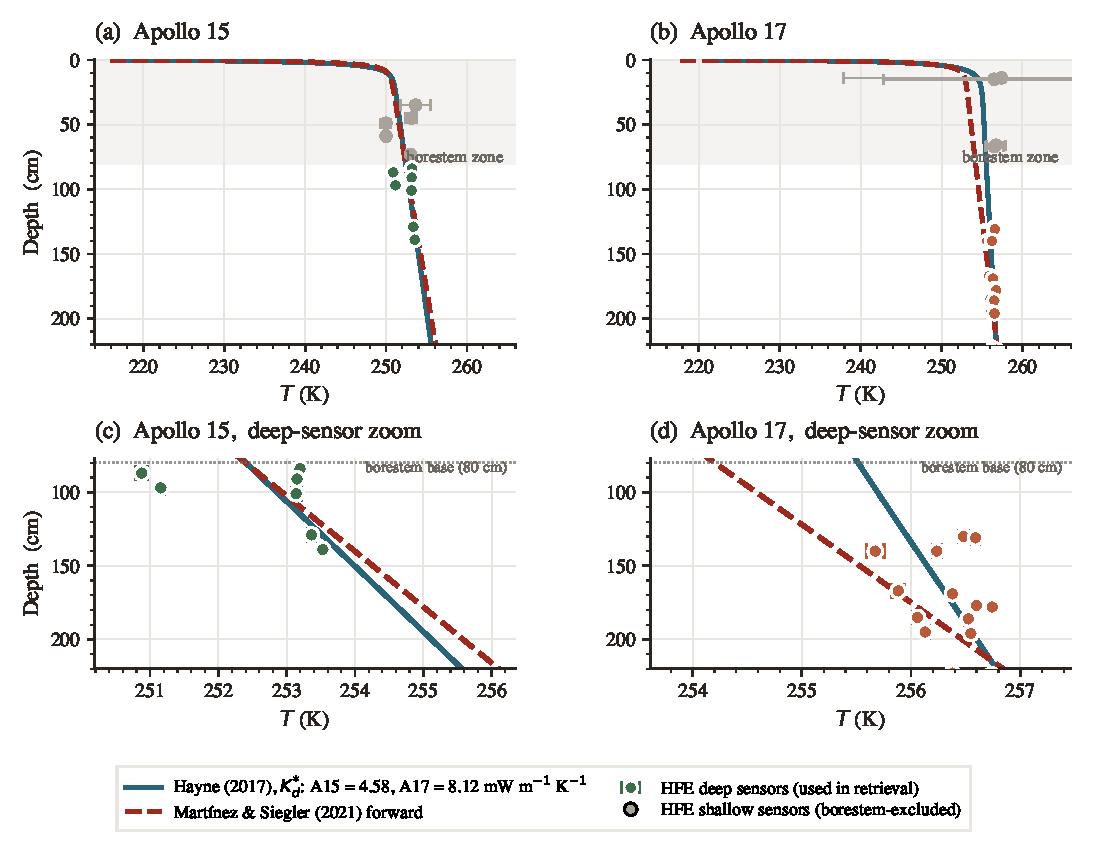
\includegraphics[width=\linewidth]{figures/fig_thermal_profiles.pdf}
\caption{\textbf{The fitted temperature profiles.} Coloured dots are the
real deep sensors; curves are the best-fit models. The bottom row zooms
in on the deep region actually used. Apollo~15 shows the
\emph{steeper} temperature rise with depth --- the signature of its
lower conductivity (and higher heat flux), since a poorer conductor
needs a steeper gradient to pass the heat (the gradient law,
Section~2.3). Apollo~17, more conductive, rises more gently.}
\label{fig:profiles}
\end{figure}

\subsection{Why these particular values make physical sense}

A conductivity of 4.6 at Apollo 15 sits comfortably between the global
average (3.4) and orbital estimates ($\sim$7), and matches what soil
porosity (how fluffy vs.\ packed it is) predicts.

Apollo 17 being $\sim$1.8 times higher is explained by two effects that
both point the same way: (1) its soil is volcanic basalt, which is
intrinsically more conductive than the highland rock at Apollo 15; and
(2) it appears slightly more tightly packed. Neither effect has to be
pushed to an extreme --- together they comfortably cover the factor of
1.8.

\begin{plainbox}
The bigger conductivity at Apollo 17 is not mysterious: it is exactly
what you would expect from denser, more volcanic soil. Two independent
soil-property arguments predict the size of the difference we measured.
\end{plainbox}

\subsection{An independent sanity check}

The retrieval only used \emph{deep} temperatures. As a completely
separate test, we checked whether the same models reproduce the
\emph{surface} temperature swing measured by an orbiting spacecraft
(Diviner). They do (Figure~\ref{fig:diviner}) --- confirming the whole
simulation chain (sunlight, day length, surface balance) is set up
correctly, independently of the deep retrieval.

\begin{figure}[t]
\centering

\includegraphics[width=\linewidth]{figures/fig_diviner_closure.pdf}
\caption{\textbf{Independent check.} Grey dots: surface temperature over
a lunar day measured from orbit. Curves: our models. The good match (a
few K over a 280\,K swing) confirms the forcing is right; this data was
not used in the retrieval.}
\label{fig:diviner}
\end{figure}

% =====================================================================
\section{Honest limits (what a critic would say)}

A good study states clearly where it could be wrong. Ours has three main
caveats, all in the manuscript:

\begin{enumerate}
\item \textbf{The absolute values lean on the assumed heat flux $Q_b$.}
      The gradient law fixes the \emph{ratio} $Q_b/K_d$, not $K_d$ by
      itself. We used the standard published $Q_b$; if those are revised,
      our $K_d$ values shift proportionally. The \emph{difference}
      between the sites is far more robust than either absolute value.
\item \textbf{Only two boreholes exist.} Two points cannot prove that
      conductivity varies smoothly across the whole Moon --- only that
      these two specific places differ. Settling the broader question
      needs new landed missions.
\item \textbf{The Apollo 17 value is sensitive to a few inputs.} Its
      precision (the error bar) is tight, but its accuracy depends on
      choices like the surface brightness coefficient; we report this
      openly in the error budget.
\end{enumerate}

\begin{plainbox}
What is rock-solid: the two sites need different conductivities, and
Apollo 17 is the more conductive one. What is conditional: the exact
numbers, which depend on the assumed heat flux and the chosen model form.
The paper is careful to say which is which.
\end{plainbox}

% =====================================================================
\section{How to run the code yourself}

The whole study regenerates from the public repository with a few
commands:

\begin{verbatim}
git clone https://github.com/rp3gregorio/Lunar-HFE.git
cd Lunar-HFE
python3 -m venv .venv && source .venv/bin/activate
pip install -e ".[dev]"

# the core retrieval (writes output/kd_retrieval_results.json):
python scripts/pipeline/retrieve_kd.py

# the figures:
python scripts/figures/make_letter_figures.py
python scripts/figures/make_results_figures.py
\end{verbatim}

\noindent A tour of the pieces:
\begin{itemize}
\item \texttt{lunar/} --- the engine. \texttt{solver.py} steps the heat
      equation in time; \texttt{equilibrium.py} is the settled-state
      solver from Section~5; \texttt{properties.py} holds the
      conductivity/density/heat formulas; \texttt{constants.py} stores
      every physical number with its literature source.
\item \texttt{scripts/pipeline/} --- the analysis: the retrieval,
      bootstrap, and all the sensitivity checks.
\item \texttt{scripts/figures/} --- the figure generators (including
      \texttt{make\_primer\_figures.py}, which made the teaching figures
      in this document).
\item \texttt{output/} --- the committed numerical results, so anyone can
      verify the paper's numbers without rerunning.
\item \texttt{docs/FLAG\_REPORT.md} --- the full record of the audit and
      the bug fix described in Section~5.
\end{itemize}

% =====================================================================
\section*{Glossary}
\addcontentsline{toc}{section}{Glossary}

\begin{description}[leftmargin=8.5em,style=nextline,font=\bfseries]
\item[Regolith] The Moon's surface layer of broken rock and dust.
\item[Thermal conductivity ($K$, $K_d$)] How easily heat passes through
  material. $K_d$ is the value deep down, where the soil is packed and
  steady. Small $=$ good insulator. Our target quantity.
\item[Basal heat flux ($Q_b$)] The steady trickle of heat rising from
  the Moon's warm interior.
\item[Diurnal skin / skin depth] The shallow zone (top few cm) where the
  day--night temperature swing is still felt; the skin depth is how far
  it reaches.
\item[Gradient ($\Delta T/\Delta z$)] How many degrees the temperature
  rises per metre of depth. Steep gradient $=$ good insulator.
\item[Heat equation] The differential equation governing how temperature
  evolves as heat flows; what the solver integrates.
\item[Boundary conditions] The rules at the two ends of the column:
  radiation balance at the surface, fixed heat flux $Q_b$ at the bottom.
\item[Retrieval] The procedure of guessing $K_d$, simulating, and
  keeping the value that best matches the data.
\item[RMSE] Root-mean-square error: a single number for the typical
  model--data disagreement, in degrees. Smaller is better.
\item[Bootstrap] Resampling the data many times to measure how uncertain
  the answer is.
\item[Equilibrium / steady state] The settled condition where the
  temperature no longer changes from one lunar day to the next.
\item[Borestem cut] Discarding sensors above 80\,cm because the probe
  stem contaminates them.
\item[HFE] Heat-Flow Experiment --- the Apollo instrument packages whose
  data we use.
\item[A15 / A17] Shorthand for the Apollo 15 and Apollo 17 sites.
\end{description}

\end{document}
